% This is samplepaper.tex, a sample chapter demonstrating the
% LLNCS macro package for Springer Computer Science proceedings;
% Version 2.21 of 2022/01/12
%
\documentclass[runningheads]{llncs}
%
\usepackage[T1]{fontenc}
% T1 fonts will be used to generate the final print and online PDFs,
% so please use T1 fonts in your manuscript whenever possible.
% Other font encondings may result in incorrect characters.
%
\usepackage{graphicx}
\usepackage{amsmath}
\usepackage{amsfonts}
\usepackage{array} % Required for \arraybackslash
% Used for displaying a sample figure. If possible, figure files should
% be included in EPS format.
%
% If you use the hyperref package, please uncomment the following two lines
% to display URLs in blue roman font according to Springer's eBook style:
%\usepackage{color}
%\renewcommand\UrlFont{\color{blue}\rmfamily}
%\urlstyle{rm}
%
\usepackage[normalem]{ulem} % Provides underlining
\usepackage{xcolor}        % For text colors

% Define the \rev command
%\newcommand{\rev}[1]{\textcolor{red}{#1}} 
\newcommand{\rev}[1]{{#1}} 

\usepackage{multirow}
%\usepackage{float}
\usepackage{algorithm}
\usepackage{algpseudocode}
\renewcommand{\algorithmicrequire}{\textbf{Input:}}
\usepackage{comment}

\begin{document}

\title{\rev{A Hybrid Approach for Pallet Loading in Ceramic Tile Industry}}

\author{Marco Taccini\inst{1}\orcidID{0009-0004-7257-473X} \and
Matheus Aguilar de Oliveira\inst{2}\orcidID{0000-0002-4671-2500} \and
André Gustavo dos Santos\inst{2}\orcidID{0000-0002-9700-9815} \and
Thiago Alves de Queiroz\inst{3}\orcidID{0000-0003-2674-3366} \and
Manuel Iori\inst{1}\orcidID{0000-0003-2097-6572}
}
%
\authorrunning{Taccini et al.}
% First names are abbreviated in the running head.
% If there are more than two authors, 'et al.' is used.
%
\institute{Department of Sciences and Methods for Engineering, University of Modena and Reggio Emilia, Reggio Emilia, Italy.\\
\email{\{marco.taccini,manuel.iori\}@unimore.it}
\and
Department of Informatics, Federal University of Viçosa, Viçosa, MG, Brazil.\\
\email{\{matheus.a.aguilar,andresantos\}@ufv.br} 
\and
Institute of Mathematics and Technology, Federal University of Catalão, Catalão, GO, Brazil.\\
\email{taq@ufcat.edu.br}
}
%
\maketitle              % typeset the header of the contribution
%
\begin{abstract}

\rev{Motivated by a real-world case study in ceramic tile production, this paper addresses the problem of determining the minimum number of pallets required to load a given set of boxes. The problem must be solved quickly to give customers an expectation of the transportation cost of their orders. In addition, not all constraints and instance data can be easily determined in advance, and the items are loaded onto the pallets by operators who mostly rely on their personal experience. Therefore, traditional model-based solution methods do not apply well, and data-driven approaches are preferable. To solve the problem, we propose a hybrid algorithm in which a machine learning technique is trained over a company dataset comprising two years of customer orders, with the aim of predicting the number of pallets required by an order. The accuracy of the machine learning technique is largely improved by including additional features, such as lower and upper bounds, in the dataset, obtained using quick optimization algorithms. The resulting hybrid algorithm has been compared with the model-based software currently used at the company, consistently providing better-quality results in shorter computing times.}

\keywords{Cutting and packing problems \and Distributor's pallet loading \and Ceramic tile \and Machine learning.}
\end{abstract}

\section{Introduction}
The global ceramic tile market has grown significantly over the past decade, with worldwide production reaching 16.8 billion square meters \cite{mecs2023}. Italy is a leading exporter, generating €7.2 billion in revenue, highlighting the sector's importance to the national economy. %
\rev{Efficient logistics optimization in the ceramic tile industry, including loading of tiles on pallets and transportation of pallets,} is crucial for cost reduction and company competitiveness. Loading operations involve transferring specified quantities of ceramic tile boxes, either of the same size or different sizes, from production pallets to shipping pallets to fulfill customers' orders. When loading pallets, the company needs to carefully consider weight and volume constraints and keep pallet stability and balance to ensure the safe transport of tiles while using the minimum number of shipping pallets.

In this paper, we handle a variant of the distributor's pallet loading problem (DPLP) \cite{Mungwattana2023} that emerges from an international ceramic tile company headquartered in Italy. The company has an e-commerce platform to receive customers' orders. As the company does not provide the transportation of the shipping pallets, customers need to collect their pallets by using their vehicles or third-party carriers. Consequently, the company should provide the number of shipping pallets associated with each order or at least predict this number accurately, especially for customers who need to contract a third-party carrier. This prediction is complex, even if using specialized software to address pallet loading problems \cite{Silva2016}, because the company faces specific constraints in its operational daily routine, necessitating extensive customization of such software. 

\rev{In this paper, we propose a hybrid approach to predict the number of shipping pallets required for a given customer order. The approach combines machine learning (ML) techniques to gain information from a large dataset of previously shipped pallets with techniques from the optimization field to enrich the dataset by quickly providing additional features such as lower and upper bounds on the number of pallets. The hybrid approach is then compared with solutions currently in use at the company, including manual operators' decisions and outputs from a given specialized software \cite{packvol}. The computational experiments show that the proposed approach is a valuable tool for the company.}

The remainder of the paper is organized as follows. Section \ref{sec2} contains a brief review of the literature related to the DPLP. Section \ref{sec3} describes the company problem with its constraints and requirements. Section \ref{sec4} presents our proposed hybrid approach. Section \ref{sec5} contains the numerical experiments on real-world instances. Finally, Section \ref{sec6} concludes the paper and provides several directions for future research. 


\section{Literature Review \label{sec2}}

The literature on cutting and packing problems is extensive. According to \cite{Sweeney1992}, the first scientific papers on these problems date back to the 1940s. The most recent surveys concern problems in one-, two-, and three-dimensions and contain detailed discussions on solution methods based on exact and heuristic approaches (see, e.g., \cite{IORI2021} and \cite{Yagiura2025}). An essential characteristic of these problems is given by the number of practical constraints they may include, such as complete shipment, conflicting items, cargo stability, load-bearing, multi-drop, and load-balancing \cite{NASCIMENTO2021}. 
Concerning pallet loading problems, \cite{Silva2016} surveyed the manufacturer's variant, in which all items are identical, and the objective is to pack the maximum number of items onto a single pallet. Besides commenting on the different data sets and solution methods, the authors emphasized that the computational complexity of this problem is still an open question. 
\rev{The DPLP, on the other hand, assumes that items are not necessarily identical and is an NP-hard problem. Its objective is to find the minimum number of pallets necessary to load all items. The DPLP is also referenced as the multi-pallet loading problem \cite{TERNO2000} and the pallet building problem \cite{Calzavara2021}.}


One of the first authors to handle the DPLP was \cite{Hodgson1982}, considering the transport of palletized cargo by the U.S. Air Force. The author proposed a dynamic programming-based algorithm and tested it on instances having 30 boxes.  
%
In \cite{TERNO2000}, the DPLP was solved using an algorithm based on branch-and-bound. The authors considered practical constraints such as weight limits, load-bearing, stability, and grouping of items.
%
In \cite{Birgin12}, the problem had no limit on the number of boxes to load, and boxes could have multiple orientations. The authors developed a recursive partitioning algorithm, which integrated a recursive five-block heuristic and an L-approach. The authors could not find an instance for which this algorithm failed in finding an optimal solution (such an instance was later found in \cite{TFW2015}). In \cite{Calzavara2021}, the DPLP emerged from a robotized task of loading boxes into layers, which were then stacked while meeting load-bearing requirements. Constraints like contiguity, visibility, and multiple orientations were considered. The authors proposed a mathematical model and a reactive greedy randomized adaptive search procedure for solving realistic, large-sized instances. A new DPLP variant in which pallets may have different sizes was handled in \cite{Mungwattana2023}. The problem emerged from a lamp and lighting manufacturing company that needed to load many carton boxes onto pallets of multiple sizes. Constraints such as load-bearing and multiple orientations were taken into consideration. 

Using artificial intelligence techniques to handle combinatorial optimization problems is a promising area of research. The survey in \cite{BENGIO2021} discussed recent advances in combining ML techniques with optimization methods to efficiently handle hard combinatorial optimization problems. The authors also commented on the benefits (e.g., speed and generalization) and challenges (e.g., training and accuracy) of using ML purely. Concerning cutting and packing problems, an increasing number of publications combine ML or artificial intelligence techniques with exact or heuristic algorithms to handle, e.g., bin packing \cite{Fang2023} and container loading problems \cite{QUE2023}. 


\section{Problem Description \label{sec3}} 


The problem under investigation is a variant of the DPLP with specific operational and product-related constraints.
\rev{After being produced, the ceramic tiles are first loaded on production pallets, which are only used for inbound logistics. An automated system then delivers the production pallets to the loading area. The company operators load the products onto shipping pallets using hydraulic machines.} The automated system is also responsible for other logistics activities inside the warehouse. As a result, products are not available simultaneously, as their arrival sequence depends on the system's decisions and the warehouse's current state. For instance, machinery downtime may alter the order in which production pallets are sent to the loading areas. Moreover, the loading area cannot have more than four production pallets at a time. Due to this space limitation, operators need to load the products onto the pallets as soon as possible. As other products arrive, operators continue loading until the shipping pallets of that order are completed before moving to the next order. \rev{When loading a shipping pallet, operators must also satisfy load requirements such as vertical stability, load-bearing, and restricted box orientations.}

Our DPLP can be formally described as follows. A customer order consists of a set \( B \) of three-dimensional boxes, each containing a given number of tiles. Each box belongs to a type \( t \in T = \{1,2,...,m\} \), corresponding to a specific tile size. A box of type \( t \) has width \( w_t \in \mathbb{Z}^{*}_{+} \), depth \( l_t \in \mathbb{Z}^{*}_{+} \), height \( h_t \in \mathbb{Z}^{*}_{+} \), and weight \( p_t \in \mathbb{Z}^{*}_{+} \). 
Let \( d_t \in \mathbb{N}\) denote the number of boxes of type \( t \) required by the order. Let \( P \) represent the set of identical shipping pallets, each with a two-dimensional loading surface of width \(W \in \mathbb{Z}^{*}_{+}\) and depth \( L \in \mathbb{Z}^{*}_{+} \). The DPLP's objective is to load all boxes requested in the order by using the minimum number of pallets. Constraints on the maximum pallet height \( H \in \mathbb{Z}^{*}_{+} \) and weight \(W_{\max} \in \mathbb{Z}^{*}_{+} \) need to be satisfied. 

Due to these complex company constraints, obtaining a solution for this DPLP variant is not easy, especially for large-sized and heterogeneous orders (i.e., composed of boxes of different sizes). \rev{Even if a DPLP solution satisfying all constraints is available, it could suffer from warehouse uncertainties, possibly making it impractical for the company operators.} Besides that, the company should give the number of pallets associated with each customer's order at the moment of purchase on its e-commerce platform. 
Therefore, the company is currently interested in a fast and accurate tool capable of predicting the number of shipping pallets, rather than solving a dedicated but time-consuming optimization problem.


\section{Hybrid Model \label{sec4}}

We propose a hybrid approach to the DPLP under investigation that considers optimization algorithms to enhance the predictive performance of an ML model. The company provided data on two years of sales and the corresponding number of pallets generated for each order. This data includes the maximum number of boxes per shipping pallet for each box \rev{size $t$, denoted by $F_t^{\max}$, and the maximum weight ($W_{\max}$) and volume ($WLH$) a shipping pallet can support.}

An initial training dataset is created from the company-provided data. We start calculating the frequency $F_{t} = d_{t} $ (i.e., the number of boxes of type $t$), the weight $W_{t} = d_{t}p_{t}$, and the volume $V_{t} = w_{t}l_{t}h_{t}d_{t}$ for each type \( t \in T \). The dataset is labeled with the number of shipping pallets $Z_j$ generated by each order $j \in \{1,...,n\}$. 
Since training on the initial dataset can take a long time, all intermediate training steps (\rev{Sections \ref{modelcomparison} - \ref{heuristicsolution}}) are conducted using a reduced dataset. The complete dataset \rev{is only used on the final computational experiments (Section \ref{sec5}).} The reduced dataset is created by randomly selecting a subset of orders from the initial dataset, resulting in a training set with about $1\over8$ of the total number of orders. 

\subsection{Machine Learning Model Selection \label{modelcomparison}} 

We developed a pipeline to train and test four different machine learning models. These models, which were chosen based on the literature review and our experience, consist of: XGBoost \cite{xgboost}, LightGBM (LGBM) \cite{lightgbm}, Random Forest, and Support Vector Machine (SVM) from scikit-learn \cite{scikitlearn}. Each model passes through a hyperparameter tuning phase on the Mean Squared Error (MSE) and Mean Absolute Error (MAE) metrics, obtained by performing a standard grid search. Table \ref{tab:grid-search-param-range} reports the hyperparameters and their possible values, besides the best values found along with MSE and MAE metrics. The possible values were defined using a trial-and-error approach and following the indications in each model documentation and the literature (see, e.g., \cite{kaggle-xgbost-tuning}). 


\begin{table}[H]
\small
\centering
\caption{Grid search results with the hyperparameter values and errors.}\label{tab:grid-search-param-range}
\begin{tabular}{|c|c|c|c|c|c|}
\hline
Model                    & Hyperparameter   & Values                      & Best Value & MSE                    & MAE                   \\ \hline \hline
\multirow{3}{*}{XGBoost} & learning\_rate   & 0.1, 0.3                    & 0.3        & \multirow{3}{*}{4.78}  & \multirow{3}{*}{1.17} \\
                         & max\_depth       & 4, 5, 6                     & 4          &                        &                       \\
                         & gamma            & 0, 0.25, 1                  & 0.25       &                        &                       \\ \hline
\multirow{2}{*}{LGBM}    & learning\_rate   & 0.005, 0.01                 & 0.01       & \multirow{2}{*}{16.49} & \multirow{2}{*}{2.58} \\
                         & num\_leaves      & 6, 8, 12, 16                & 16         &                        &                       \\ \hline
\multirow{3}{*}{\begin{tabular}[c]{@{}c@{}}Random\\ Forest\end{tabular}} & max\_features & sqrt, log2, None & None & \multirow{3}{*}{13.61} & \multirow{3}{*}{2.26} \\
                         & max\_depth       & 3, 6, 9                     & 9          &                        &                       \\
                         & max\_leaf\_nodes & 3, 6, 9                     & 9          &                        &                       \\ \hline
\multirow{2}{*}{SVM}     & C                & 0.1, 1, 10, 100, 1000       & 100        & \multirow{2}{*}{35.89} & \multirow{2}{*}{3.45} \\
                         & gamma            & 1, 0.1, 0.01, 0.001, 0.0001 & 0.0001     &                        &                       \\ \hline
\end{tabular}
\end{table}

The results in Table \ref{tab:grid-search-param-range} show that XGBoost outperforms the other models regarding the MSE and MAE values. Consequently, we decided to use only XGBoost in the following steps. We also decided to perform a deeper tuning of this model's hyperparameters. Table \ref{tab:grid-search-deep-param} contains the outcome of this additional tuning test, which leads to better MSE and MAE values for the XGBoost model.


% \usepackage{multirow}
\begin{table}
\small
\centering
\caption{XGBoost tuning with the best hyperparameter values and errors.}\label{tab:grid-search-deep-param}
\begin{tabular}{|c|c|c|c|c|}
\hline
Hyperparameter     & Values              & Best Value & MSE                   & MAE                   \\ \hline \hline
learning\_rate     & 0.01, 0.1, 0.2, 0.3 & 0.3        & \multirow{6}{*}{1.11} & \multirow{6}{*}{0.43} \\
gamma              & 0, 0.1, 0.5         & 0.1        &                       &                       \\
max\_depth         & 3, 6, 10            & 6          &                       &                       \\
min\_child\_weight & 0, 1, 3, 5          & 0          &                       &                       \\
subsample          & 0.5, 1              & 0.5        &                       &                       \\
colsample\_bytree  & 0.5, 1              & 1          &                       &                       \\ \hline
\end{tabular}
\end{table}


\subsection{Features Optimization \label{featureoptimization}} 

After successfully fine-tuning the XGBoost model, we investigated the importance of each feature in the reduced dataset. This analysis reveals that columns $W_{t}$ and $V_{t}$, for $t \in T$, are marginally contributing to the model's predictions, as shown in Figure \ref{fig:feat-weights-1}. Furthermore, tile sizes that appear less frequently in the dataset exhibit higher error rates, as shown in Figure \ref{fig:mse-vs-freq}. 

\begin{figure}
\centering
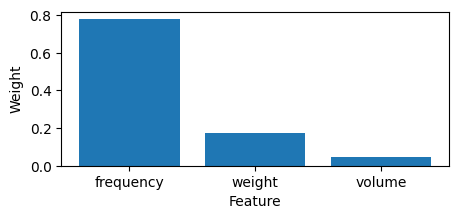
\includegraphics[width=.55\textwidth]{figures/feat-weights-1.png}
\caption{Importance of the feature weights in the XGBoost model.} \label{fig:feat-weights-1}
\end{figure}

\begin{figure}[H]
\centering
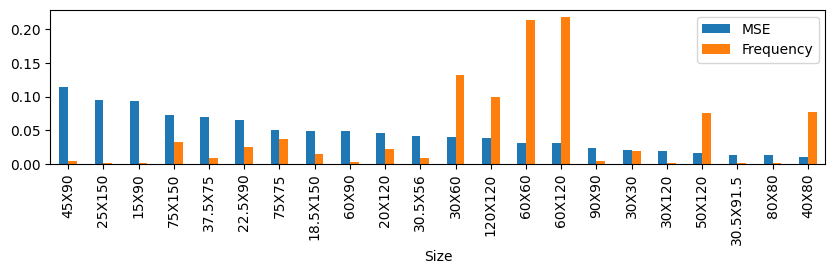
\includegraphics[width=0.8\textwidth]{figures/mse-vs-freq.png}
\caption{MSE and frequency values ($F_t$), normalized and sorted by decreasing MSE.} \label{fig:mse-vs-freq}
\end{figure}


These results allow the removal of less informative features, such as the size-grouped weight $W_t$ and volume $V_t$. 
\rev{At the same time, we introduce more general order-aggregated features, as follows. Let $O$ be the set of orders we need to process, and let $o \in O$ be a given order. We determine the total number of boxes $F_o = \sum_{t=1}^{m}{F_{t}}$, the total weight $W_{o} = \sum_{t=1}^{m}{W_{t}}$, the total volume $V_{o} = \sum_{t=1}^{m}{V_{t}} $, the average box weight $W_{avg} = {W_{o} \over F_{o}}$, and the average box volume $V_{avg} = {V_{o} \over F_{o}}$.} Figure \ref{fig:feat-weights-2} shows how these new features impacted the predictive capability of the XGBoost model.

\begin{figure}
\centering
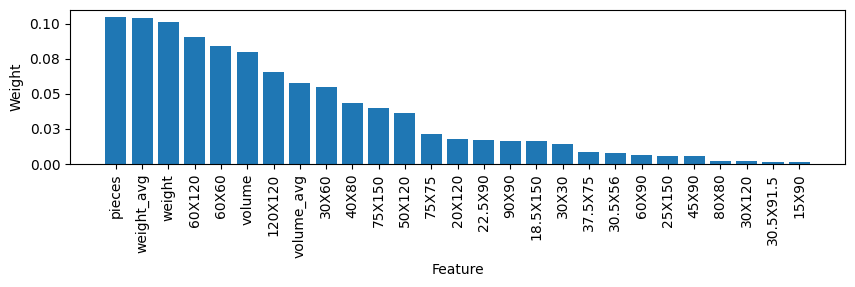
\includegraphics[width=0.8\textwidth]{figures/feat-weights-2.png}
\caption{Importance of the new order-aggregated features in the XGBoost model.} \label{fig:feat-weights-2}
\end{figure}


In the set $O$ of orders, we observe that predicting the number of shipping pallets for homogeneous orders, defined $O_h$, which consist of only one type of box, and $O_{full}$ ones, which require only production pallets regardless of the types, is straightforward for the model. In this way, we divided results into two groups: one containing all available orders $O$ and another excluding these simpler orders $O_{mix} = O - (O_h \cup O_{full}$). With this strategy, we evaluated the model in both scenarios, preventing simple orders to improve the metrics and resulting in premature conclusions. Table \ref{tab:new-cols-comparison} summarizes the model's performance before and after including the new features.


\begin{table}[H]
\centering
\caption{MSE and MAE values for each group of orders and the dataset structures $S_1$ (original) and $S_2$ (enriched with additional features).}\label{tab:new-cols-comparison}
\begin{tabular}{c|cc|cc|}
\cline{2-5}
\multicolumn{1}{l|}{}       & \multicolumn{2}{c|}{MSE}         & \multicolumn{2}{c|}{MAE}         \\ \hline \hline
\multicolumn{1}{|c|}{Dataset structure} & \multicolumn{1}{c|}{$O$} & $O_{mix}$ & \multicolumn{1}{c|}{$O$} & $O_{mix}$ \\ \hline
\multicolumn{1}{|c|}{$S_1$} & \multicolumn{1}{c|}{1.01} & 1.38 & \multicolumn{1}{c|}{0.42} & 0.53 \\ \hline
\multicolumn{1}{|c|}{$S_2$} & \multicolumn{1}{c|}{0.36} & 0.47 & \multicolumn{1}{c|}{0.24} & 0.31 \\ \hline
% \multicolumn{1}{|c|}{$S_3$} & \multicolumn{1}{c|}{0.24} & 0.32 & \multicolumn{1}{c|}{0.19} & 0.20 \\ \hline
\end{tabular}
\end{table}


\subsection{Incorporation of Optimization-based Features \label{heuristicsolution}}
    

Aiming to reduce the errors further, three additional features (i.e., $HS_1$, $HS_2$, and $HS_3$) computed with quick algorithms are introduced into the training dataset. To ensure computational efficiency, the proposed algorithms have the worst-case time complexity of at most $O(F_{o}^{2})$, where $F_{o}$ is the total number of boxes in the customer's order. The proposed algorithms are as follows:

\begin{itemize}
    \item $HS_1$: calculated as $HS_1 = \max{(\lceil{\sum_{t=1}^{m} {W_t}\over {W_{\max}}} \rceil,\lceil{\sum_{t=1}^{m} {V_t}\over {WLH}} \rceil)}$. \rev{This can be interpreted as the value of the linear relaxation lower bound (LB);}
    
    \item $HS_2$: calculated as $HS_2 = \sum_{t=1}^m \lceil{ {F_t} \over {{F_t^{\max}}} }\rceil$, where $F_{t}^{\max}$ is the maximum number of boxes of type $t$ that can be loaded onto a pallet. This is, instead, an upper bound (UB) for the DPLP instance, computed by considering that all pallets are built with only homogeneous tiles (and this can easily be done by satisfying vertical stability and load bearing constraints);

    \item $HS_3$: described in Algorithms \ref{alg:hs3alg} and \ref{alg:trypackalg}. This algorithm loads pallets by stacking layers of same-sized boxes, starting with those having the largest area until the pallet limits are reached. Once full, it begins a new pallet and continues until all boxes are packed. \rev{This may be seen as a quick heuristic solution approach, but, in fact, it does not consider vertical stability and load bearing constraints, and hence it only provides an approximation function of the minimum number of pallets.}
    
\end{itemize}

\begin{algorithm}[H]
\caption{\textsc{HS3} - constructive heuristic to give the number of shipping pallets} \label{alg:hs3alg}
\begin{algorithmic}[1]
\State $pallets \gets 1$ \Comment{Pallet estimation}
\For{$t \in \textsc{sorted}(T)$} \Comment{Iterate over box types sorted by decreasing base area}
    \While {$d_t > 0$} \Comment{Boxes of type $t$ left to pack}
        \If{$w - p_t < 0 \textbf{ OR } h - h_t < 0 \textbf{ OR } \text{no space to pack one box}$}
            \State $x, y, w, h \gets W, L, W_{\max}, H$ \Comment{Restart using an empty pallet}
            \State $pallets \gets pallets + 1$
        \EndIf
        \State $b \gets \lfloor{w \over {p_t}}\rfloor$ \Comment{How many boxes can be packed based on weight}
        \State $q, d_x, d_y \gets \textsc{tryPack}(b, w_t, l_t, x, y) $ \Comment{Try to pack directly}
        \State $q_2, d_{x2}, d_{y2} \gets \textsc{tryPack}(b, l_t, w_t, x, y) $ \Comment{Try rotating to pack}
        \If{$q < q_2 \textbf{ OR } (q = q_2 \textbf{ AND } p_xp_y < p_{x2}p_{y2})$}
            \State $q, d_x, d_y \gets q_2, d_{x2}, d_{y2}$ \Comment{Choose to pack more boxes, then more area}
        \EndIf
        \State $d_t, w, h \gets d_t - q, w - p_tq, h - h_t$ \Comment{Pack boxes, update weight and height}
        %\State $d_t \gets d_t - q$ \Comment{Pack boxes}
        %\State $w \gets w - p_tq$ \Comment{Update available weight}
        %\State $w , h\gets w - p_tq, h - h_t$ \Comment{Update available weight and height}
        %\State $h \gets h - h_t$ \Comment{Update available height}
        \State $x, y \gets d_x, d_y$ \Comment{Update dimensions for next layer}
    \EndWhile
\EndFor
\State \textbf{return} $pallets$
\end{algorithmic}
\end{algorithm}

\begin{algorithm}[H]
\caption{\textsc{tryPack}} \label{alg:trypackalg}
\begin{algorithmic}[1]
\Require{$b, b_x, b_y, l_x, l_y$} \Comment{Boxes to pack, box and layer dimensions}
\State $X \gets \min(b, \lfloor{l_x \over {b_x}}\rfloor)$ \Comment{Maximum number of boxes in x-dimension}
\State $Y \gets \min(b, \lfloor{l_y \over {b_y}}\rfloor)$ \Comment{Maximum number of boxes in y-dimension}
\State $q, d_x, d_y \gets 0, 0, 0$ \Comment{Best quantity and new layer dimensions}
\For{$x \in \{1 \dots X\}$} \Comment{Test all number of boxes in x-dimension}
    \State $y \gets \min(Y, \lceil{b \over x}\rceil)$ \Comment{How many rows in y-dimension will be needed}
    \If{$q < \min(b, xy) \textbf{ OR } (q = \min(b, xy) \textbf{ AND } d_x d_y < b_x b_y x y)$}
        \State $q, d_x, d_y \gets \min(b, xy), b_x x, b_y y$
    \EndIf
\EndFor
\State \textbf{return} $q, d_x, d_y$
\end{algorithmic}
\end{algorithm}

Table \ref{tab:finaldataset} describes the final structure $S_3$ of the training dataset, which now includes the three additional optimization-based features. 
%
Compared with Table \ref{tab:new-cols-comparison}, the MSE and MAE values for the dataset structure $S_3$ are 0.24 and 0.19 for $O$, and 0.32 and 0.26 for $O_{mix}$, respectively, representing a considerable improvement in the accuracy of the model. 

\begin{table} [H]
\centering
\caption{Final training dataset structure $S_3$.} 
\label{tab:finaldataset}
\begin{tabular}{|
>{\centering\arraybackslash}p{0.8cm}|
>{\centering\arraybackslash}p{0.8cm}|
>{\centering\arraybackslash}p{0.5cm}|
>{\centering\arraybackslash}p{0.8cm}|
>{\centering\arraybackslash}p{1cm}|
>{\centering\arraybackslash}p{1cm}|
>{\centering\arraybackslash}p{1cm}|
>{\centering\arraybackslash}p{0.8cm}|
>{\centering\arraybackslash}p{0.8cm}|
>{\centering\arraybackslash}p{0.8cm}|
>{\centering\arraybackslash}p{0.8cm}|
>{\centering\arraybackslash}p{0.8cm}|
>{\centering\arraybackslash}p{0.8cm}|
}
\hline
$j$ &
$F_{1}$ &
$\dots$ &
$F_{m}$ &
$F_{o}$ &
$W_{o}$ &
$V_{o}$ &
$W_{avg}$ &
$V_{avg}$ &
$HS_{1}$ &
$HS_{2}$ &
$HS_{3}$ &
$Z_{j}$ \\ \hline \hline
1 &  10 &  $\dots$ &  3 &  25 &  250 &  500 &  10 &  20 & 5 & 9 & 8 & 7 \\ \hline
$\dots$ &  $\dots$ &  $\dots$ & $\dots$ &  $\dots$ &  $\dots$ & $\dots$ &  $\dots$ &  $\dots$ & $\dots$ & $\dots$ & $\dots$ & $\dots$ \\ \hline
$n$ &  7 &  $\dots$ &  0 & 13 & 195 &  65 & 15 &  5 & 2 & 4 & 3 & 3 \\ \hline
\end{tabular}
\end{table}


\section{Computational Experiments \label{sec5}} 

\rev{All the codes were implemented in Python 3.10 and executed in a computer with an Intel Core i5-1135G7 2.40 GHz processor, 8 GB of RAM, and Linux Mint 21 Cinnamon as the operating system.} 
We evaluate the XGBoost model considering the structure $S_3$ (i.e., the one enriched with the additional optimization-based features) and the complete two-year dataset with all orders. This corresponds to our hybrid approach. 
In Table \ref{tab:finalresultstable}, we observe the impact of the two groups $O_h$ and $O_{full}$ on the training phase. Consequently, we train the model using the structure $S_3$, first including all orders $O$ and then keeping only mixed orders $O_{mix}$ (which we recall is equal to $O - (O_h \cup O_{full})$).

\begin{table}[H]
\centering
\caption{MSE and MAE values for each group of orders and the dataset structure $S_3$.}
\label{tab:finalresultstable}
\begin{tabular}{ccc|cc|cc|}
\cline{4-7}
\multicolumn{1}{c}{}            &                       &  & \multicolumn{2}{c|}{MSE}         & \multicolumn{2}{c|}{MAE}         \\ \hline \hline
\multicolumn{1}{|c|}{Groups of orders} &
  \multicolumn{1}{c|}{Orders} &
  Training Time (min) &
  \multicolumn{1}{c|}{$O$} &
  $O_{mix}$ &
  \multicolumn{1}{c|}{$O$} &
  $O_{mix}$ \\ \hline
\multicolumn{1}{|c|}{$O$} & \multicolumn{1}{r|}{166391} & \multicolumn{1}{c|}{54.79} & \multicolumn{1}{c|}{0.22} & 0.73 & \multicolumn{1}{c|}{0.11} & 0.33 \\ \hline
\multicolumn{1}{|c|}{$O_{mix}$} & \multicolumn{1}{r|}{40533} & \multicolumn{1}{c|}{ 26.90}  & \multicolumn{1}{c|}{0.25} & 0.76 & \multicolumn{1}{c|}{0.12} & 0.33 \\ \hline
\end{tabular}
\end{table}

As reported in Table \ref{tab:finalresultstable}, applying the model to all orders $O$ yields slightly better results compared to using $O_{mix}$. However, using only $O_{mix}$ can reduce the training time by around 51\% while keeping satisfactory predictive results. 

We next compare in Table \ref{tab:comparisonresults} the proposed hybrid approach with PackVol \cite{packvol}, a specialized software the company uses to solve the DPLP heuristically. PackVol was configured by the company employees to satisfy the specific operational constraints of the DPLP as closely as possible. This means that PackVol is not able to capture some constraints. For example, as mentioned in Section \ref{sec3}, ceramic tiles of a given order are not all available simultaneously due to the warehouse's current state. As a result, PackVol could underestimate the number of pallets. We also present the number of pallets obtained from the company operators for comparison purposes. This experiment considers 30 real instances, consisting of 30 orders randomly selected among the heterogeneous orders made in 2024 (which are not included in the training set). 
The real instances $I$ are all heterogeneous, and are sorted by increasing number of box types $m$. Its maximum value is 6 since 99.32\% of the orders in the training dataset contain six or fewer types. Table \ref{tab:comparisonresults} contains the instance number and the solution value (i.e., number of shipping pallets) obtained with PackVol, the proposed hybrid approach, and the company operators. We assume the operators' solution is the basis for comparison, so the rows ``Diff.'' contain the difference with such a solution for each instance. \rev{Positive values indicate the usage of more pallets, which could be acceptable. Negative values indicate fewer pallets in the solution and could represent additional logistic issues for customers (e.g., the need for contracting ``on the flight'' an extra vehicle).}


\begin{table}[H]
\scriptsize
\caption{Results for the 30 real instances and comparison among the different methods.}
\label{tab:comparisonresults}
\begin{tabular}{|c|c|c|c|c|c|c|c|c|c|c|c|c|c|c|c|c|c|c|c|c|c|c|c|c|c|c|c|c|c|c|}
\hline
Inst. & 1 & 2 & 3 & 4 & 5 & 6 & 7  & 8 & 9 & 10 & 11 & 12 & 13 & 14 & 15 & 16 & 17 & 18 & 19 & 20 & 21 & 22 & 23 & 24 & 25 & 26 & 27 & 28 & 29 & 30 \\ \hline \hline
\# types & 2 & 2 & 2 & 2 & 2 & 2 & 3  & 3 & 3 & 3  & 3  & 3  & 4  & 4  & 4  & 4  & 4  & 4  & 5  & 5  & 5  & 5  & 5  & 5  & 6  & 6  & 6  & 6  & 6  & 6  \\ \hline
Company	&	2	&	6	&	4	&	1	&	6	&	2	&	22	&	5	&	5	&	8	&	10	&	7	&	5	&	8	&	9	&	7	&	15	&	6	&	26	&	9	&	28	&	2	&	13	&	10	&	22	&	10	&	22	&	21	&	10	&	16	\\	\hline	\hline	
PackVol	&	1	&	6	&	4	&	1	&	6	&	2	&	22	&	5	&	3	&	8	&	10	&	6	&	4	&	6	&	8	&	7	&	15	&	6	&	25	&	8	&	27	&	4	&	13	&	6	&	18	&	8	&	21	&	19	&	10	&	14	\\		
Diff.	&	-1	&	0	&	0	&	0	&	0	&	0	&	0	&	0	&	-2	&	0	&	0	&	-1	&	-1	&	-2	&	-1	&	0	&	0	&	0	&	-1	&	-1	&	-1	&	2	&	0	&	-4	&	-4	&	-2	&	-1	&	-2	&	0	&	-2	\\	\hline	\hline		
Hybrid	&	2	&	7	&	4	&	1	&	6	&	2	&	22	&	5	&	5	&	9	&	11	&	7	&	6	&	7	&	9	&	7	&	16	&	7	&	26	&	9	&	27	&	3	&	13	&	10	&	21	&	10	&	22	&	20	&	12	&	16	\\		
Diff.	&	0	&	1	&	0	&	0	&	0	&	0	&	0	&	0	&	0	&	1	&	1	&	0	&	1	&	-1	&	0	&	0	&	1	&	1	&	0	&	0	&	-1	&	1	&	0	&	0	&	-1	&	0	&	0	&	-1	&	2	&	0	\\	\hline	

\end{tabular}
\end{table}


Observing the results in Table \ref{tab:comparisonresults}, PackVol achieves an MSE of 2.13 and an MAE of 0.93, whereas our hybrid approach achieves significantly better results, with 0.50 and 0.43 values of MSE and MAE, respectively. These outcomes highlight that our approach outperforms PackVol in both metrics, demonstrating its capability to predict the number of pallets following \rev{ the real context of the company with its operational requirements and workflows}.
Another important aspect is the computation time required by the proposed approach. Although the training phase may be time-consuming, after training, it solved all instances in just 0.016 seconds, while PackVol required around one second per instance. \rev{From Table \ref{tab:comparisonresults}, we can also observe that PackVol returns solutions different from those by the company in 16 cases, returning fewer pallets for 15 cases and achieving a largest deviation of -4 pallets. This may bring issues for customers. On the other hand, the hybrid approach returns solutions that differ from the company ones for just 12 instances, returning fewer pallets for only 4 of them and having the largest deviation of just 2 pallets. These values confirm that our approach, trained on real-world data, effectively models the problem constraints and results in accurate predictions.}

\section{Concluding Remarks \label{sec6}}

\rev{We proposed a hybrid approach composed of machine learning and optimization components to predict the number of pallets required to ship an order of ceramic tiles. We evaluated four machine learning models, and after fine-tuning, we selected XGBoost. Its performance was improved by adding new features that capture general information about the company's operational constraints. We also incorporated three measures obtained by quick optimization algorithms, leading to significant reductions in both MSE and MAE values. The resulting hybrid approach obtained better results than PackVol, the specialized model-based software currently used at the company. 

The computational experiments highlight that our hybrid approach, once it is trained on real-world data, is fast and well-suited for the company-specific operational constraints. It allows more accurate and practical predictions than PackVol, resulting in more solutions equal to the ones obtained by the company operators and a reduced number of solutions requiring fewer pallets. This is remarkably achieved without feeding the approach with any direct information about the pallet loading constraints (i.e., stability, load-bearing requirements, and orientation), making the approach a very flexible tool.}

\rev{Future research could propose new features to the hybrid approach (e.g., solutions obtained with heuristics based on local search). Another interesting research avenue is to work on a more general problem, considering pallets of different sizes, which will lead to a more challenging objective function. We finally plan to test the approach to other related pallet loading, cutting, and packing problems, as well as scheduling problems \cite{BLM2024,QM2020}.}


\subsubsection{\ackname} 

We acknowledge financial support from the National Council for Scientific and Technological Development (CNPq) [grant n. 405369/2021-2, 408722/2023-1, 315555/2023-8, 444679/2024-3, and 407005/2024-2], the State of Goi\'as Research Foundation (FAPEG), and the National Recovery and Resilience Plan (NRRP), Mission 04 Component 2 Investment 1.5–NextGenerationEU, Call n. 3277 dated 30/12/2021, Award n.: 0001052 dated 23/06/2022. We are also grateful to the company, which has provided us with relevant information, feedback, and data.

\bibliographystyle{splncs04}
\bibliography{bibliography}
\end{document}
